%%%%%%%%%%%%%%%%%%%%%%%%%%%%%%%%%%%%%%%%%%%%%%%%%%%%%%%%%%%%%%%%%%%%%%%%%%%%
%% Text Area: 8in (include Runningheads) x 5in
%% ws-ijmpa.tex   :   01-07-2026
%% Tex file to use with ws-ijmpa.cls written in LaTeX2e.
%% The content, structure, format and layout of this style file is the
%% property of World Scientific Publishing Co. Pte. Ltd.
%% Copyright 2026 by World Scientific Publishing Co.
%% All rights are reserved.
%%%%%%%%%%%%%%%%%%%%%%%%%%%%%%%%%%%%%%%%%%%%%%%%%%%%%%%%%%%%%%%%%%%%%%%%%%%%
%%

%\documentclass[wsdraft]{ws-ijmpa}
\documentclass{ws-ijmpa}

\usepackage{siunitx}
\usepackage{tikz-feynman}
\usepackage{slashed}

\usepackage[super]{cite}
\usepackage{xcolor}
\usepackage[verbose,hypertexnames=false]{hyperref}
\hypersetup{colorlinks=false,allbordercolors=blue,pdfborderstyle={/S/U/W 1}}
% \label, \ref and \cite commands are highly recommended

\begin{document}

\markboth{Liang Wei}{Multi-Messenger Observation of NGC 1068}

%%%%%%%%%%%%%%%%%%%%% Publisher's Area please ignore %%%%%%%%%%%%%%%
%
\catchline{}{}{}{}{}
%
%%%%%%%%%%%%%%%%%%%%%%%%%%%%%%%%%%%%%%%%%%%%%%%%%%%%%%%%%%%%%%%%%%%%

\title{Research on Phenomenology of HNL\\
  and Possible Signals in Multi-Messenger Observation
}

\author{Liang Wei}

\address{Physics Department, East China Normal University, No. 500 Dongchuan Rd.\\
  Shanghai, China\\
  weiliang1503@gmail.com}

\author{Jianhong Ruan}

\address{Physics Department, East China Normal University, No. 500 Dongchuan Rd.\\
  Shanghai, China\\
  jhruan@phy.ecnu.edu.cn}

\maketitle

% \begin{history}
% \received{Day Month Year}
% \revised{Day Month Year}
% \accepted{Day Month Year}
% \published{Day Month Year}
% \end{history}

\begin{abstract}
  Recently, the IceCube detector has identified AGN NGC 1068 as a
  point source of high-energy neutrinos, while the $\gamma$ ray observation
  exceeds the prediction of electromagnetic cascade models. This suggests
  some of the $\gamma$ ray energy can be transported outside from being
  attenuated. In this paper we propose HNL, Heavy Neutral Leptons, as
  a way to explain this observation. We first review the origin of HNL
  theory, calculating the phenomenology behavior of certain processes
  related to $p-\gamma$ and $p-p$ neutrino production, then use it to try to
  explain the $\gamma$ ray observation of AGN NGC 1068, and several other
  astronomical observations.
\end{abstract}

\keywords{HNL; multi-messenger; NGC 1068}

% \ccode{PACS numbers: 03.65.$-$w, 04.62.+v}

\section{Introduction}

As advancements are made in astronomical observations, different types
of new signals have became observable, along side with gravitational
waves and wider range of electro-magnetic signals, neutrino signals
are now observed by IceCube, which has recently spotted AGN NGC 1068 as
a point source of neutrino
flux around energy of $\qty{1}{TeV}$ \cite{icecube2022evidence}, and several other experiments, such as
KM3NeT/ARCA, while still under
construction, has observed a neutrino signal which possibly has energy
as high as \qty{220}{PeV}.\cite{km3net2025observation}

Further more, neutrino has always been the strange one in Standard Model (SM),
because of its tiny mass, thus weak coupling with the Higgs field, is
considered some what unnatural. This leads neutrino and the origin of its
small mass to be considered as a key to Beyond Standard Model Physics (BSM),
such as Heavy Neutral Lepton (HNL) being candidate of dark mater.
A lot of experiments on the earth is working on finding possible signals
coming from BSM theories.\cite{PhysRevLett.103.241802} Although no definite
signal has been observed, they do provide a solid constrain on the parameter
space of possible BSM theories, for HNL with $\qty{3}{MeV} < m_N < \qty{19.5}{MeV}$, the
mixing angle with muon neutrino is constrained roughly as $|U_{\mu N}|^2 \lesssim 10^{-4}$.
\cite{bryman2019constraints}

And, in the observation of NGC 1068 done by IceCube, when comparing with
theoretical predictions \cite{murase2020hidden} based on corona cascade models, exceeds the
prediction of observed $\gamma$-ray flux around \qty{10}{GeV} energy. This suggests
that the hidden core of NGC 1068 has some process to transport more,
electro-magnetic energy out. Axion is one option \cite{pant2024constraining},
another option is HNL, which is discussed in this paper. Before NGC 1068,
there are already attempts to combine multi-messenger observations in
favor of constraining BSM theories.\cite{PhysRevLett.58.1490,
  PhysRevD.94.085012, Magill_2018}.

This paper is structured as follows. In Section , we outline the basic of HNL
theory originating from neutrino mass, and calculate its phenomenology
properties, while taking polarization into account. In Section , we investigate
the multi-messenger observation results of NGC 1068, try to explain the
exceeding $\gamma$-ray flux. Conclusion is in Section .

\section{ISS Model}

To explain the tiny mass of neutrino, a bunch of models known as Seesaw
Mechanisms are proposed. For Type-I Seesaw model, we have
\begin{equation}
  m_\nu = \frac{m_D^2}{M_R}, \; m_N = M_R, \; |U|^2 = \left( \frac{m_D}{M_R} \right)^2
\end{equation}
Where $m_D$ is the Dirac mass of neutrino, and $M_R$ is the Majorana mass
of the added right-handed neutrino field. For a sufficiently natural $m_D$
and $m_R$, the mixing angle $|U|^2$ is always too small which makes observation
impossible. How every by introducing another fermionic field, the mass
matrix becomes
\begin{equation}
  \begin{pmatrix}
    \overline{\nu_L} & \overline{\nu_R^c} & \overline{S^c}
  \end{pmatrix}
  \begin{pmatrix}
    0   & m_D & 0   \\
    m_D & 0   & M   \\
    0   & M   & \mu
  \end{pmatrix}
  \begin{pmatrix}
    \nu_L^c \\
    \nu_R   \\
    S
  \end{pmatrix}
\end{equation}
The new parameter $\mu$ stands for potential lepton number violation, which should
be small. The basic properties of neutrino and a pseudo-dirac fermion pair, which can be treated
as a fermion because of the small $\mu$, are
\begin{equation}
  m_\nu = \mu \frac{m_D^2}{M^2}, \; m_N = M, \; |U|^2 = \frac{m_\nu}{\mu}
\end{equation}

\section{HNL Production}

Such HNL particles only interact through its mixed part of SM neutrino,
which means those process which produces SM neutrino, if not prohibited
by phase space, will also produce HNL at the same time.

\subsection{Pion decay}
Under the condition of AGN, $p-p$ and $p-\gamma$ processes are though
to be the origin of high energy cosmic rays.\cite{Murase_2023} Those
processes creates a large number of pions, and the decay of high-energy
pions turns into high-energy cosmic rays, including neutrinos, $\gamma$-rays.
\cite{kelner2006energy}

After introducing HNL particle mixing with SM neutrino, charged pions can decay
into HNL particles, intermediated by W bosons.
\begin{figure}[htbp]
  \centering
  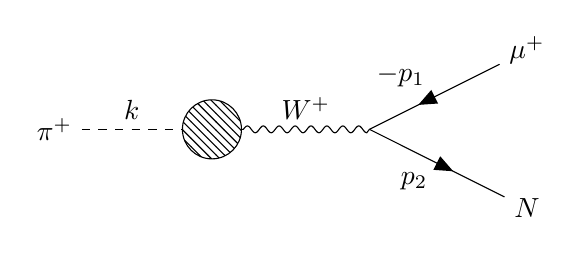
\begin{tikzpicture}
    \begin{feynman}
      \vertex [blob] (a) at (0, 0) {};
      \vertex (b) at (2, 0);
      \vertex (i1) at (-2, 0) {$\pi^+$};
      \vertex (f1) at (4, 1) {$\mu^+$};
      \vertex (f2) at (4, -1) {$N$};
      \diagram* {
      (i1) -- [scalar, edge label=$k$] (a),
      (a) -- [boson, edge label=$W^+$] (b),
      (f2) -- [anti fermion, edge label=$p_2$] (b) -- [anti fermion, edge label=$-p_1$] (f1),
      };
    \end{feynman}
  \end{tikzpicture}
  \caption{Feynman diagram of $\pi^+$ decaying into $\mu^+$ and massive HNL particle.}
\end{figure}
By slightly modifying the process of SM pion decay, we find that the decay width
to HNL is
\begin{equation}
  \frac{\Gamma_{\pi \to \mu N}}{\Gamma_{\pi \to \mu \nu}} =
  |U_{\mu}|^2 \times \rho_\pi (m_N) \label{eq:pion_HNL_rho}
\end{equation}
Where
\begin{align}
   & \rho_\pi (m_N) = \frac{(m_\pi^2 (m_\mu^2 + m_N^2) - (m_\mu^2 - m_N^2)^2) \sqrt{\lambda(m_\pi^2, m_\mu^2, m_N^2)}}{m_\mu^2 (m_\pi^2 - m_\mu^2)^2} \label{eq:rho_pi} \\
   & \lambda(x, y, z) = x^2 + y^2 + z^2 - 2xy - 2yz - 2zx
\end{align}
It is useful to determine the helicity of the HNL particle, since
it will play a role in the angular dependence when working on the
decay of HNL. In the pion rest frame we have
\begin{equation}
  % \Gamma_{\pi \to N}^{(s)} \propto (m_\mu^2 + m_N^2) m_\pi^2 - (m_\mu^2 - m_N^2)^2 - s \cdot (m_\mu^2 - m_N^2) \sqrt{\lambda(m_\pi^2, m_\mu^2, m_N^2)}
  {\Gamma_{(s)}} \sim {(m_\mu^2 + m_N^2) m_\pi^2 - (m_\mu^2 - m_N^2)^2 - s(m_\mu^2 - m_N^2) \sqrt{\lambda(m_\pi^2, m_\mu^2, m_N^2)}} \label{eq:hnl_hel_pion}
\end{equation}
Where $s$ is the helicity of HNL, and $s=+1$ for right-handed polarized HNL particle.
There are no differences in angular dependence for different helicity end
states, since pion is unpolarized. After boosting to the lab frame,
we must account for the polarization change on the HNL particles,
thus for a pion spectrum $J(E_\pi)$, we get
\begin{equation}
  Q_{N}^{(s)}(E_N) = \int_{\frac{E_N}{\lambda_{max}}}^{\infty} J(E_\pi) |U_{\mu}|^2 \rho_\pi \times r_{(s)}(E_\pi, E_N) \times \frac{d E_\pi}{\lambda_{max} E_\pi} \label{eq:hnl_spec_from_pion}
\end{equation}
Where
\begin{align}
   & \lambda_{max}       = \frac{E_{N,max}}{E_\pi} = \frac{m_\pi^2 - m_\mu^2 + m_N^2 + \sqrt{\lambda(m_\pi^2, m_\mu^2, m_N^2)}}{2 m_\pi^2}       \\
   & \cos\theta_r        = \frac{E_N(m_\pi^2 - m_\mu^2 + m_N^2) - 2 E_\pi m_N^2}{\sqrt{(E_N^2 - m_N^2) \, \lambda(m_\pi^2, m_\mu^2, m_N^2)}}     \\
   & r_{(s)}(E_\pi, E_N) = \frac{\Gamma_{(s)}\frac{1 + \cos\theta_r}{2} + \Gamma_{(-s)}\frac{1 - \cos\theta_r}{2}}{\Gamma_{(s)} + \Gamma_{(-s)}}
\end{align}
Here we assume $E_\pi \gg m_\pi$ to simplify the boost process.

\subsection{Muon decay}
Muons will decay into HNL particles through a similar process as
they decay into $\nu_\mu$. We find the decay width of $\mu^- \to N e^- \bar{\nu}_e$ has the same
form as the process of $\tau$ decay which has been studied
\cite{Bondarenko_2018}, since this process is symmetric between
$\mu$ and $\tau$, which is
\begin{equation}
  \frac{\Gamma_{\mu \to N}}{\Gamma_{\mu \to \nu_\mu}} = |U_{\mu}|^2 \times \rho_\mu(m_N)
\end{equation}
Where
\begin{equation}
  \rho_\mu(m_N) = - r_N^8 + 8 r_N^6 - 24 r_N^4 \ln(r_N) - 8 r_N^2 + 1 \label{eq:rho_mu},\;\;
  r_N = m_N / m_\mu
\end{equation}
And the spectrum of HNL particle under muon rest frame, separated by polarization, is
\begin{align}
  \frac{d\Gamma}{dE} = \frac{G_F^2}{24 \pi^3} |U_\mu|^2 \times |\mathbf{p}| \cdot [ & 3 (m_\mu^2 + m_N^2) E - 4 m_\mu E^2 - 2 m_N^2 m_\mu \nonumber                   \\
                                                                                    & - s \cdot |\mathbf{p}| (m_N^2 + 3 m_\mu^2 - 4 m_\mu E) ] \label{eq:mu_HNL_spec}
\end{align}
Several examples are plotted in Fig.~\ref{fig:muon_decay_spec}.

\begin{figure}[t]
  \centerline{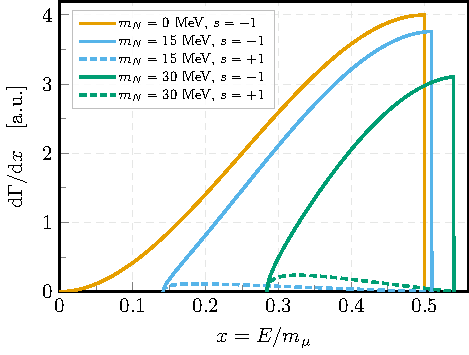
\includegraphics{../julia_plots/muon_decay_spectrum.pdf}}
  \caption{Energy spectrum of HNL when muons decay into HNLs in muon rest frame.
  Normalized under $m_N = 0$, which
  basically resembles SM neutrino, with no right-handed product exists.
  When $m_N$ increases, shape of the spectrum stays roughly the same,
  but the max energy increases while the total decay
  width decreases, and more right-handed HNLs, though still a small
  fraction, will be produced.}
  \label{fig:muon_decay_spec}
  \alttext{HNL Spectrum of Muon Decay Separated by Helicity}
\end{figure}

Though one can keep the muon polarization and calculate the angular
dependence of how many different helicity HNL particles will be produced
while the angle respect to muon polarization changes, we will
simply ignore the muon polarization here as we assume that the
magnetic environment
of AGN will wipe the polarization out.

% For different HNL energy, we have
% \begin{align}
%   \frac{d\Gamma_{(s)}}{dE} \sim \; &3 (m_\mu^2 + m_N^2) E - 4 m_\mu E^2 - 2m_N^2 m_\mu \nonumber \\
%   &- s \cdot |\mathbf{p}| (m_N^2 + 3 m_\mu^2 - 4 m_\mu E) 
% \end{align}
For a given muon spectrum, we have

\begin{align}
  Q_N^{(s)}(E_N) = \int_{E}^{+\infty} &d E_\mu \, Q_\mu(E_\mu) |U_\mu|^2 \rho_\mu \nonumber \cdot \int_{x^-}^{x^+}  \frac{d x}{E_\mu \sqrt{x^2 - \frac{m_N^2}{m_\mu^2}}} \nonumber \\
  & \cdot \left(\frac{1 + \cos\theta_r}{2} g_N^{(s)}(x) + \frac{1 - \cos\theta_r}{2} g_N^{(-s)}(x)\right)
\end{align}
Where
\begin{align}
  x^+ &= \frac{m_N^2 + m_\mu^2}{2 m_\mu^2}, \; x^- = \frac{1}{2} \left( \frac{E_N}{E_\mu} + \frac{E_\mu}{E_N} \cdot \frac{m_N^2}{m_\mu^2}\right) \\
  \cos\theta_0 &= \frac{1}{\sqrt{x^2 - \frac{m_N^2}{m_\mu^2}}}\left(\frac{E_N}{E_\mu} - x\right) \\
  \cos\theta_r &= \frac{E_\mu}{\sqrt{E_N^2 - m_N^2}}\left( \sqrt{x^2 - \frac{m_N^2}{m_\mu^2}} + x \cos\theta_0\right)
\end{align}
While $g^{(s)}_N(x)$ is normalized as
\begin{equation}
  \int^{x^+}_{x^-} dx \sum_{s=\pm 1} g^{(s)}_N(x) = 1
\end{equation}

\section{HNL Decay}
Straight-forwardly, HNL particles under ISS model will , and will
only, decay into other leptons. Possible products are $\nu_\mu e^- e^+$
and $\nu_\mu \nu_l \bar{\nu}_l$. These processes are well studied\cite{Bondarenko_2018},
we can recall the decay width for each process as
\begin{align}
  \Gamma_{N \to 3\nu}          & = \frac{G_F^2 m_N^5}{192 \pi^3} \times |U_\mu|^2 \label{eq:HNL_3nu_decay}               \\
  \Gamma_{N \to \nu e \bar{e}} & = \frac{G_F^2 m_N^5}{192 \pi^3} \times |U_\mu|^2 \times C_1^e \label{eq:HNL_nuee_decay}
\end{align}
Where
\begin{equation}
  C_1^e = \frac{1}{4}\left(1 - 4 \sin^2 \theta_W + 8 \sin^4 \theta_W\right)
\end{equation}
To simplify the problem we will ignore electron mass, and $3\nu$ end state
has taken all different flavor combinations into account.

Thus the branch ratio of HNL particle processing a visible decay
is
\begin{equation}
  BR_{N \to \nu e \bar{e}} = \frac{C_1^e}{1 + C_1^e} \approx 0.11
\end{equation}
The energy loss is pretty significant. Only one tenth of HNL
decays will be observable.
The angular and energy distributions of electrons/positrons are
\begin{align}
  g_e^{(1)}(x, \cos{\theta}) = & \frac{8}{C_1^e} \cdot x^2 \cdot \{ [(4 - 16 s_W^2 + 64 s_W^4) x - (1 - 4 s_W^2 + 28 s_W^4)] \cos{\theta} \nonumber   \\
                               & - (4 - 16 s_W^2 + 64 s_W^4) x + (3 - 12 s_W^2 + 36 s_W^4) \} \label{eq:g_e_p2}                                       \\
  g_e^{(2)}(x, \cos{\theta}) = & \frac{16}{C_1^e} \cdot x^2 \cdot \{ [(6 - 24 s_W^2 + 32 s_W^4) x - (3 - 12 s_W^2 + 14 s_W^4)] \cos{\theta} \nonumber \\
                               & - (6 - 24 s_W^2 + 32 s_W^4) x + (3 - 12 s_W^2 + 18 s_W^4) \} \label{eq:g_e_p3}
\end{align}
Where  $x = E_e / m_N$, $s_W = \sin{\theta_W}$. $\theta$ is the
angle between the out-going electron and initial HNL spin.

To get the total electron spectrum from a given HNL spectrum, we
integral over the HNL spectrum and get
\begin{align}
  Q_e^{(Lab)}(E) = BR_{N \to \nu e \bar{e}} \cdot \int_{E}^{+\infty} &d E_N \, Q_N^{(s)}(E_N) \nonumber \\
  &\cdot \int_{\frac{E}{2 E_N}}^{\frac{1}{2}}  \frac{d x}{x E_N} \, \sum_{i=1,2} g_e^{(i)}(x, s (\frac{E}{x E_N} - 1))
\end{align}
Combining with \ref{eq:g_e_p2} and \ref{eq:g_e_p3}, the remaining
integral is
\begin{equation}
  \int_{E}^{+\infty} \frac{d E_N}{E_N} \, Q_N^{(s)}(E_N) [16 y^3 - 27 y^2 + 11 -  s \cdot (32 y^3 - 63 y^2 + 36 y - 5) ]
\end{equation}
Where $y=E/E_N$, and $\theta_W$ no-longer appears in this formula.

\section{Multi-Messenger Observation of NGC 1068}

\section{General Appearance}
Contributions to {\it International Journal of Modern Physics A}
are to be in American English. Authors are encouraged to have their
contribution checked for grammar. American spelling should be
used. Abbreviations are allowed but should be spelled out in full when
first used. Integers ten and below are to be spelled out.  Italicize
foreign language phrases (e.g.~Latin, French).  Upon acceptance,
authors are required to submit their data source file including
postscript files for figures.

The text is to be typeset in 10 pt roman, single spaced with
baselineskip of 13~pt. Text area (including copyright block)
is 8 inches high and 5 inches wide for the first page.  Text area
(excluding running title) is 7.7 inches high and 5 inches wide for
subsequent pages.  Final pagination and insertion of running titles
will be done by the publisher.

\section{Running Heads}
Please provide a shortened runninghead (not more than eight words) for
the title of your paper. This will appear on the top right-hand side
of your paper.

\section{Major Headings}
Major headings should be typeset in boldface with the first
letter of important words capitalized.

\subsection{Subheadings}
Subheadings should be typeset in boldface italic and capitalize
the first letter of the first word only. Section numbers to be in
boldface roman.

\subsubsection{Subsubheadings}
Typeset subsubheadings in medium face italic and capitalize the
first letter of the first word only. Section numbers to be in
roman.

\subsection{Numbering and spacing}
Sections, subsections and subsubsections are numbered in
Arabic.  Use double\break spacing before all section headings, and
single spacing after section headings. Flush left all paragraphs
that follow after section headings.

\subsection{Lists of items}
Lists may be laid out with each item marked by a bullet:
\begin{itemlist}
  \item item one,
  \item item two.
\end{itemlist}
Items may also be numbered in lowercase roman numerals:
\begin{romanlist}[(ii)]
  \item item one,
  \item item two.
  \begin{romanlist}[(b)]
    \item Lists within lists can be numbered with lowercase
    roman letters,
    \item second item.
  \end{romanlist}
\end{romanlist}

\section{Equations}
Displayed equations should be numbered consecutively in each
section, with the number set flush right and enclosed in
parentheses
\begin{equation}
  \mu(n, t) = \frac{\sum^\infty_{i=1} 1(d_i < t, N(d_i)
    = n)}{\int^t_{\sigma=0} 1(N(\sigma) = n)d\sigma}\,.
  \label{diseqn}
\end{equation}

Equations should be referred to in abbreviated form,
e.g.~``Eq.~(\ref{diseqn})'' or ``(\ref{diseqn})''. In multiple-line
equations, the number should be given on the last line.

For multiline equations, prefer using \verb|align| or \verb|align*| instead of \verb|eqnarray|.
\begin{align}
  g(x) & = \sum_{k=1}^{N} y_k g(x_k) \nonumber                    \\
       & = \sum_{k=1}^{N} y_k \sum_{l=1}^{M} b_{kl} w_l \nonumber \\
       & = \sum_{k=1}^{N} \sum_{l=1}^{M} b_{kl} y_k w_l
\end{align}

Displayed equations are to be centered on the page width.
Standard English letters like x are to appear as $x$
(italicized) in the text if they are used as mathematical
symbols. Punctuation marks are used at the end of equations as
if they appeared directly in the text.

\section{Theorem Environments}

\begin{theorem}\label{thm1}
  Theorems$,$ lemmas$,$ propositions$,$ corollaries are to be numbered
  consecutively in the paper or in each section. Use italic for the
  body and upper and lower case boldface$,$ for the declaration.
\end{theorem}

\begin{remark}\label{rem1}
  Remarks, examples, definitions are to be numbered
  consecutively in the paper or in each section. Use roman for the
  body and upper and lower case boldface$,$ for the declaration.
\end{remark}

\begin{proof}
  The word `Proof' should be typed in boldface. Proofs
  should end with\break
  a box.
\end{proof}

\section{Figures}
Figures are to be embedded in the text nearest their first reference
and sequentially numbered in Arabic numerals. The caption must be
placed below the figure (see Fig.~\ref{f1}) and typeset in 8 pt roman with
baselineskip of 10 pt. Use double spacing between a caption and the
text that follows immediately.

\begin{figure}[t]
  \centerline{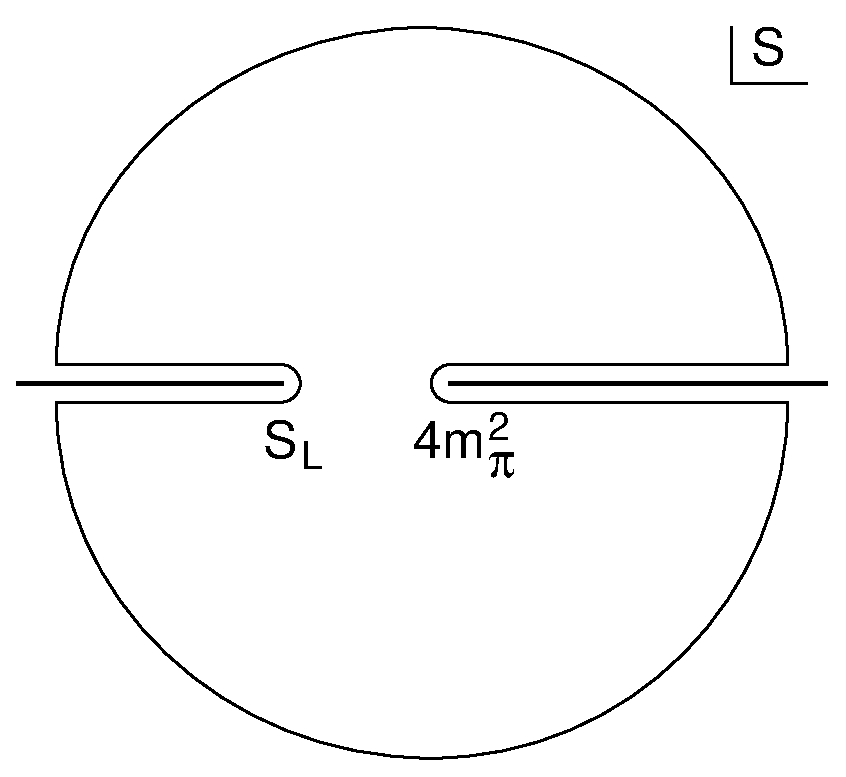
\includegraphics[width=3.8cm]{ijmpaf1}}
  \caption{A schematic illustration of dissociative recombination. The
    direct mechanism, 4m$^2_\pi$ is initiated when the
    molecular ion S$_{\rm L}$ captures an electron with
    kinetic energy.}
  \label{f1}
  \alttext{Description of the figure}
\end{figure}

Figures should be black and white (or half-tone) and of a good
resolution and sharpness. Compressed formats, such as JPEG, should not
use heavy compression, which introduces undesirable artifacts. Bitmap
figures, such as photographs or half-tone images, should be at least
300 dpi (TIFF, BMP or JPEG). Vector (line-art) figures, such as
charts and technical drawings, should be 600--1200 dpi (EPS, PS,
PDF). The native formats of software packages will not be permitted.

Previously published material must be accompanied by written
permission from the author and publisher.

\section{Tables}
Tables should be inserted in the text as close to the point of
reference as possible. Some space should be left above and below
the table.

Tables should be numbered sequentially in the text in Arabic
numerals. Captions are to be centralized above the tables (see
Table~\ref{ta1}).  Typeset tables and captions in 8 pt roman with
baselineskip of 10 pt.

\begin{table}[ph]
  \tbl{Comparison of acoustic for frequencies for piston-cylinder problem.\label{ta1}}
  {\begin{tabular}{@{}cccc@{}} \toprule
      Piston mass      & Analytical frequency & TRIA6-$S_1$ model  & \% Error        \\
                       & (Rad/s)              & (Rad/s)                              \\
      \colrule
      1.0\hphantom{00} & \hphantom{0}281.0    & \hphantom{0}280.81 & 0.07            \\
      0.1\hphantom{00} & \hphantom{0}876.0    & \hphantom{0}875.74 & 0.03            \\
      0.01\hphantom{0} & 2441.0               & 2441.0\hphantom{0} & 0.0\hphantom{0} \\
      0.001            & 4130.0               & 4129.3\hphantom{0} & 0.16            \\
      \botrule
    \end{tabular}}
\end{table}

If tables need to extend over to a second page, the continuation of
the table should be preceded by a caption, e.g.~``{\it Table 2.}
$(${\it Continued}$)$''.

\section{Footnotes}
Footnotes should be numbered sequentially in superscript
lowercase roman letters.\footnote{Footnotes should be
  typeset in 8 pt roman at the bottom of the page.}

% \section{About References and their Formats}
% References are to be listed in the order cited in the text in Arabic
% numerals. They should be listed according to the style shown in the
% References. Typeset references in 9 pt roman.

% It is recommended that each cited publication is labeled with a unique reference number. Format that contains multiple/grouped citations, e.g. ``A. David, {\it Int. J. Phys.} {\bf 18}, 11150 (2000); {\bf 18}, 22350 (2003); J. John, {\it ibid.} {\bf 6}, 11204 (2010)'', is not encouraged.

% References in the text can be typed in superscripts,
% e.g.: ``$\ldots$ have proven\cite{autbk,edbk,rvo} that
% this equation $\ldots$'' or after punctuation marks:
% ``$\ldots$ in the statement.\cite{rvo}'' This is
% done using LaTeX command: ``\verb|\cite{name}|''.

% When the reference forms part of the sentence, it should not
% be typed in superscripts, e.g.: ``One can show from
% Ref.~\refcite{autbk} that $\ldots$'', ``See
% Refs.~\citen{jpap,colla,autbk}, \refcite{rvo}
% and \refcite{pro} for more details.''
% This is done using the LaTeX
% command: ``Ref.~\verb|\citen{name}|''.

\section*{Acknowledgments}
This section should come before the References. Dedications and funding
information may also be included here.

\section*{ORCID}
You are encouraged to include in your user information the ORCID (\url{https://orcid.org/}) or register for one if you don't have it. This ID will help to identify you in the researcher community and make it easier to keep track of all your publications.
Please provide a valid ORCID here, e.g.,

\noindent Josiah Carberry - \url{https://orcid.org/0000-0002-1825-0097}

\noindent Rajesh Babu - \url{https://orcid.org/0009-0006-0415-6880}

\appendix

\section{Appendices}
Appendices should be used only when absolutely necessary. They
should come before the References. If there is more than one
appendix, number them alphabetically. Number displayed equations
occurring in the Appendix in this way, e.g.~(\ref{app1}),\break
(\ref{app2}), etc.
\begin{eqnarray}	%A.1
  \begin{array}{rcl}
    g_{\mu_1\mu_2}      & = & g_{axby}=-\displaystyle{\epsilon_{abc}}{4\pi}\,
    \frac{(x-y)^c}{|x-y|^3}\,,                                                \\[8pt]
    h_{\mu_1\mu_2\mu_3} & = & \epsilon^{\alpha_1 \alpha_2 \alpha_3}
    g_{\mu_1\alpha_1}g_{\mu_2\alpha_2}g_{\mu_3\alpha_3}
  \end{array}
  \label{app1}
\end{eqnarray}
with
\begin{align}	%A.2
  \epsilon^{\alpha_1 \alpha_2 \alpha_3} = \epsilon^{b_1y_1b_2y_2cx} =
  \epsilon^{b_1b_2c}\delta(x-y_1)\delta(x-y_2)\,.
  \label{app2}
\end{align}

\bibliographystyle{ws-ijmpa}
\bibliography{ref}

% \begin{thebibliography}{0}

% \bibitem{jpap} R. Loren and D. B. Benson, {\it J. Comput.
% System Sci.} {\bf 27}, 400 (1983), \url{https://doi.org/10.1016/0022-0000(83)90050-8}.

% \bibitem{lee} M. Lee, {\it Int. J. Phys.} {\bf 18}, 255 (2010) [Erratum: {\it ibid.} {\bf18}, 440 (2010)].

% \bibitem{colla} OPAL Collab. (G. Abbiendi {\it et al}.),
% {\it Eur. J. Phys. C\/} {\bf 11}, 217 (1999), \url{https://doi.org/10.1007/s100529900181}.

% \bibitem{autbk} C. M. Wang, J. N. Reddy and K. H. Lee, Buckling relationships, in
% {\it Shear Deformable Beams and Plates} (Elsevier, Oxford, 2000), p.~201.

% \bibitem{edbk} T. Tel, in {\it Experimental Study and Characterization
% of Chaos}, ed. Hao Bailin (World Scientific, Singapore, 1990), p.~149,
% \url{https://doi.org/10.1142/1000}.

% \bibitem{rvo} L. Aron, M. Botella and T. Lubart,  Culinary arts: Talent and their development, eds. R. F. Subotnik, P. Olszewski-Kubilius and F. C. Worrell, {\it The Psychology of High Performance$:$ Developing Human Potential into Domain-Specific Talent} (American Psychological Association, 2019), pp. 345--359, \url{https://doi.org/10.1037/0000120-016}.

% \bibitem{seri} Eds. M. Andreas and B. Zimmermann, {\it Crisis on Stage$:$ Tragedy and Comedy in Late Fifth-Century Athens}, Trends in Classics, Vol. 13  (De Gruyter, 2012).

% \bibitem{pro} R. Loren, J. Li and D. B. Benson, Deterministic
% flow-chart interpretations, in {\it Proc. 3rd Int. Conf.
% Entity-Relationship Approach}, eds. C. G. Davis and R. T. Yeh
% (North-Holland, Amsterdam, 1983), p.~421.
% \end{thebibliography}

\end{document}